\themaE
\graphicspath{{../../S24_Representer_le_pave_et_le_cylindre/Images/}}

\chapter{Représenter le pavé\\et le cylindre}
\label{S24}


%Cube
\newcommand{\cubiso}[2]     
   {\rput(#1,#2) 
      {\psset{fillstyle=solid}
       \pspolygon[fillcolor=purple!80](0,0)(2;90)(2;30)(2;-30)
       \pspolygon[fillcolor=lightgray](2;-30)(3.464;0)(4;30)(2;30)
       \pspolygon[fillcolor=teal](2;90)(2;30)(4;30)(3.464;60)}}


%%%%%%%%%%%%%%%%%%%%%%%%%%%%%%
%%%%%%%%%%%%%%%%%%%%%%%%%%%%%%
\begin{autoeval}
   \small
   \begin{enumerate}
      \item Il construire et met en relation une représentation en perspective cavalière et un patron d'un pavé droit, d'un cylindre. 
   \end{enumerate}
\end{autoeval}

\begin{prerequis}
   \begin{itemize}
      \item[\com] Construire et mettre en relation des représentations des solides suivants : pavé droit et cylindre (perspective cavalière, patrons).
      \item[\com] Utiliser un logiciel de géométrie dynamique pour représenter des solides.
   \end{itemize}
\end{prerequis}

\vfill

\begin{debat}[Débat : la perspective]
   La {\bf perspective cavalière} est un outil qui permet de représenter sur une feuille de papier des objets en volume sans point de fuite.
   Cette représentation était utilisée pour la conception des fortifications militaires. Le \og cavalier \fg{} était un promontoire de terre situé en arrière des fortifications et qui permettait de voir par-dessus la ligne des ouvrages de défense, et donc de voir les ouvrages des assaillants et ainsi d'anticiper leurs plans offensifs. D'autres perspectives sont utilisées notamment pour les arts : le perspective par {\bf point de fuite} et la {\bf perspective isométrique} par exemple.
   \begin{center} 
      {\psset{Decran=20,viewpoint=10 5 10,unit=0.45}
      \begin{pspicture}(-5,-4.5)(5,5)
         \psSolid[fcol=0 (red) 1 (Aquamarine) 2 (Bittersweet) 3 (ForestGreen) 4 (Goldenrod) 13 (GreenYellow) 40 (Mulberry), object=cube,mode=3]
      \end{pspicture}
      \begin{pspicture}(-5,-4)(5,5)
         \psSolid[fcol=0 (gray) 2 (Lavender) 3 (SkyBlue) 11 (LimeGreen) 12 (Brown) 23 (OliveGreen) 22 (Yellow) , object=cylindre,h=4,ngrid=4 10](0,0,-2)
      \end{pspicture}}  
   \end{center}
   \bigskip
   \begin{cadre}[B2][J4]
      \begin{center}
         Vidéo : \href{https://www.yout-ube.com/watch?v=zCIxdOCQiZg}{\bf Comment dessiner des illusions d'optique 3D}, chaîne YouTube {\it Simple drawing tutorial}.
      \end{center}
   \end{cadre}
\end{debat}


%%%%%%%%%%%%%%%%%%%%%%%%%%%%%%%%%%%%
%%%%%%%%%%%%%%%%%%%%%%%%%%%%%%%%%%%%
\activites

\begin{activite}[Patrons !]
   {\bf Objectifs :} tracer le patron d'un pavé droit, d'un cylindre, d'une pyramide, d'un cône, puis construire ces solides.
   \begin{QCM}
      \begin{enumerate}
         \item Citer les solides présents dans cette représentation en perspective cavalière d'un chateau. \par \medskip
            \pointilles \par \medskip
            \pointilles \medskip
          \item En se répartissant le travail dans votre groupe, construire une maquette de ce château en vraie grandeur. \\
          Pour cela, il faudra tracer le patron de chacun des solides, les assembler puis le décorer ;-)
      \end{enumerate}
      {\psset{unit=0.9}
      \begin{pspicture}(-1,-1.5)(17,14)
         \psset{fillstyle=solid}
         \psframe*[linecolor=Black!70](0,0)(4,10)
         \pspolygon*[linecolor=Black!50](4,0)(4,10)(5.5,11.5)(5.5,7)(5,6.5)(5,1)
         \pcline{<->}(0,-0.5)(4,-0.5) \lput*{:U}{\ucm{4}}
         \pcline{<->}(-0.5,0)(-0.5,10) \lput*{:U}{\ucm{10}}
         \pcline{<->}(4,9.5)(5.5,11) \lput*{:U}{\ucm{4}}
         \psframe*[linecolor=Khaki](1.25,7.25)(2.75,8.75)
         \pspolygon*[linecolor=FireBrick](0,10)(4,10)(2.75,13)
         \pspolygon*[linecolor=FireBrick!50](4,10)(5.5,11.5)(2.75,13)
         \pcline{<->}(-0.25,10.25)(2.5,13.25) \lput*{:U}{\ucm{4}}
         \psframe*[linecolor=SaddleBrown](4.5,0.5)(13,6.5)
         \pspolygon*[linecolor=SaddleBrown!50](4.5,6.5)(5,7)(13,7)(13,6.5)
         \pcline{<->}(4.5,0.25)(13,0.25) \lput*{:U}{\ucm{8}}
         \pcline{<->}(4.25,6.75)(4.75,7.25) \lput*{:U}{\ucm{2}}
         \psframe*[linecolor=Gold](8,0.5)(10,4)
         \psellipse*[linecolor=Gold](9,4)(1,0.75)
         \psframe*[linecolor=Black!70](13,0.25)(17,10.25)
         \psellipse*[linecolor=Black!70](15,0.25)(2,0.75)
         \pcline{<->}(13,-0.75)(17,-0.75) \lput*{:U}{\ucm{4}}
         \psframe*[linecolor=Khaki](14.25,7.25)(15.75,8.75)
         \pspolygon*[linecolor=FireBrick](13,10.25)(17,10.25)(15,13.25)
         \psellipse*[linecolor=FireBrick](15,10.25)(2,0.5)
         \pcline{<->}(12.75,10.5)(14.7,13.35) \lput*{:U}{\ucm{4}}
      \end{pspicture}}
   \end{QCM}
\end{activite}

\vfill\hfill{\footnotesize\it D'après une activité du site m@th et tiques d'Yvan Monka : \href{https://www.maths-et-tiques.fr/images/M_images/chateaufort.jpg}{\og Le château fort \fg}}.


%%%%%%%%%%%%%%%%%%%%%%%%%%%%%%%%%%%%
%%%%%%%%%%%%%%%%%%%%%%%%%%%%%%%%%%%%
\cours 

%%%%%%%%%%
\section{Définitions}

\begin{definition}
   \begin{itemize}
      \item La représentation en \textbf{perspective cavalière} d'un solide de l'espace est une technique de dessin permettant de représenter un solide sur une surface à deux dimensions en respectant le parallélisme.
      \item Le \textbf{patron} d'un solide est une surface plane d'un seul tenant qui, par pliage, permet de reconstituer le solide sans recouvrement de ses faces.
      \item Si le solide n'est pas un polyèdre, on parle de {\bf développement}. \\ [-8mm]
   \end{itemize}
\end{definition}

\medskip

Un patron se dessine en dépliant mentalement le solide.

\begin{exemple}  
   {\psset{fillstyle=solid,unit=0.3}
   \begin{pspicture}(-13,-4)(5,6)  
      \pspolygon[fillcolor=A2](-5.38,-3.26)(-1.46,-3.74)(-2.88,-1.66)(-6.74,-1.04)
\pspolygon[fillcolor=yellow!50](-1.06,-1.36)(4.36,0.74)(3.94,-1.66)(-1.46,-3.74)
\pspolygon[fillcolor=B2](-6.54,-0.46)(-5.24,3.82)(0.12,5.9)(-1.22,1.66)
\pspolygon[fillcolor=A2](4.48,1.22)(0.64,1.82)(0.12,-0.90)(4.36,0.74)
\pspolygon[fillcolor=yellow!50](0.12,-0.90)(-1.22,1.66)(-6.54,-0.46)(-6.27,-1.12)(-2.88,-1.66)(-2.55,-2.15)(-1.11,-1.68)(-1.06,-1.36)
\pspolygon[fillcolor=B2](-1.46,-3.74)(-2.55,-2.15)(-1.11,-1.68)
   \end{pspicture}}
\correction
   {\psset{fillstyle=solid,unit=0.7}
   \begin{pspicture}(-2.5,0)(6,4.25)
      \psframe[fillcolor=B2](-1,1)(1,3.5)
      \psframe[fillcolor=yellow!50](1,1)(2,3.5)
      \psframe[fillcolor=B2](2,1)(4,3.5)
      \psframe[fillcolor=yellow!50](4,1)(5,3.5)
      \psframe[fillcolor=A2](2,3.5)(4,4.5)
      \psframe[fillcolor=A2](2,1)(4,0)
   \end{pspicture}}
\end{exemple}

\bigskip

Le patron ou le développement d'un solide n'est pas unique, il dépend de la manière dont on le déplie.


%%%%%%%%%%%%%%%%%%%
\section{Représentations graphiques}

\begin{center}
   {\psset{unit=0.5}
   \small
   \hautab{1.5}
   \begin{CLtableau}{0.9\linewidth}{3}{c}
      \hline
      & Pavé (droit) & Cylindre (de révolution) \\
      \hline
      \rotatebox{90}{Perspective cavalière \quad} 
      &
      {\psset{unit=1.2}
      \begin{pspicture}(-3,-0.75)(9,1.5)
         \pspolygon(0,0)(4,0)(5,1)(5,4)(1,4)(0,3)
         \psline(0,3)(4,3)(4,0)
         \psline(4,3)(5,4)
         \psline[linestyle=dashed](0,0)(1,1)(5,1)
         \psline[linestyle=dashed](1,1)(1,4)
         \psdots[linecolor=red](2,0)(3,1)(2,3)(3,4)
         \psdots[dotstyle=square*,linecolor=blue](0,1.5)(4,1.5)(1,2.5)(5,2.5)
         \psdots[dotstyle=triangle*,linecolor=teal](0.5,0.5)(0.5,3.5)(4.5,0.5)(4.5,3.5)
      \end{pspicture}}
      &
      {\psset{unit=1.2}
      \begin{pspicture}(-4,-0.5)(8,2)
         \psellipse[linecolor=A1](1.6,4)(1.6,0.5)
         \psellipticarc[linestyle=dashed,linecolor=A1](1.6,0)(1.6,0.5){0}{180}
         \psellipticarc[linecolor=A1](1.6,0)(1.6,0.5){180}{0}
         \psline(0,0)(0,4)  
         \psline(3.2,0)(3.2,4)
         \psdots[linecolor=red](0,2)(3.2,2)
      \end{pspicture}} \\
      \hline
      \rotatebox{90}{Patron ou développement \qquad\qquad}
      &
      {\psset{unit=1.2}
      \begin{pspicture}(-1,-1.25)(12,2.75)
         \pspolygon(2,0)(5,0)(5,2)(10,2)(10,6)(5,6)(5,8)(2,8)(2,6)(0,6)(0,2)(2,2)
         \psframe(2,2)(5,6)
         \psline(7,2)(7,6)
         \psdots[linecolor=red](0,4)(2,4)(5,4)(7,4)(10,4)
         \psdots[dotstyle=square*,linecolor=blue](3.5,0)(3.5,2)(3.5,6)(3.5,8)(8.5,2)(8.5,6)
         \psdots[dotstyle=triangle*,linecolor=teal](1,2)(1,6)(2,1)(2,7)(5,1)(5,7)(6,2)(6,6)
      \end{pspicture}}
      &
      {\psset{unit=1.2}
      \begin{pspicture}(-1,-3.25)(12,7.5)
         \psframe(0,0)(10,4)
         \psline[linecolor=A1](0,0)(10,0)
         \psline[linecolor=A1](0,4)(10,4)
         \pscircle[linecolor=A1](2,5.6){1.6}
         \pscircle[linecolor=A1](6,-1.6){1.6}
         \psdots[linecolor=red](0,2)(10,2)
      \end{pspicture}} \\
      \hline
   \end{CLtableau}}
\end{center}


%%%%%%%%%%%%%%%%%%%%%%%%%%%%%%%%%
%%%%%%%%%%%%%%%%%%%%%%%%%%%%%%%%%
\exercicesbase

%\begin{colonne*exercice}

\begin{exercice} %1
   Terminer la représentation en perspective cavalière des trois pavés et du cylindre suivants :
   \begin{center}
      {\psset{unit=0.5}
      \begin{pspicture}(-1,-1)(30,6)
         \psgrid[subgriddiv=1,gridlabels=0pt,gridcolor=lightgray](-1,-1)(30,6)
         \psset{linewidth=0.7mm}
         \psline(0,2)(0,0)(2,0) % cube
         \psline[linestyle=dashed](0,0)(1,1)
         \psline(5,0)(5,4)(8,4)(10,5) % pavé
         \psline[linestyle=dashed](12,0)(13,2)(21,2) % pavé plat
         \psline[linestyle=dashed](13,2)(13,4)
         \psline(23,1)(23,4) % cylindre
         \psellipticarc(26,1)(3,0.5){180}{0}
      \end{pspicture}}
   \end{center}
\end{exercice}

\begin{corrige}
   \ \\ [-5mm]
   {\psset{unit=0.35}
      \begin{pspicture}(-1,-1)(12,6.7)
         \psgrid[subgriddiv=1,gridlabels=0pt,gridcolor=lightgray](-1,-1)(12,6)
         \psset{linewidth=0.4mm}
         \psline(0,2)(0,0)(2,0) % cube
         \psline[linestyle=dashed](0,0)(1,1)
         \psline[linecolor=blue](2,0)(3,1)(3,3)(1,3)(0,2)(2,2)(2,0)
         \psline[linecolor=blue](2,2)(3,3)         
         \psline[linestyle=dashed,linecolor=blue](3,1)(1,1)(1,3)
         \psline(5,0)(5,4)(8,4)(10,5) % pavé haut
         \psline[linecolor=blue](5,0)(8,0)(10,1)(10,5)(7,5)(5,4)
         \psline[linecolor=blue](8,0)(8,4)    
         \psline[linestyle=dashed,linecolor=blue](5,0)(7,1)(10,1)
         \psline[linestyle=dashed,linecolor=blue](7,1)(7,5)
      \end{pspicture} \\
      \begin{pspicture}(10,-1)(30,7)
         \psgrid[subgriddiv=1,gridlabels=0pt,gridcolor=lightgray](10,-1)(30,6)
         \psset{linewidth=0.4mm}
         \pspolygon[linecolor=blue](12,0)(20,0)(21,2)(21,4)(13,4)(12,2) % pavé plat
         \psline[linecolor=blue](12,2)(20,2)(21,4)
         \psline[linecolor=blue](20,2)(20,0)         
         \psline[linestyle=dashed](12,0)(13,2)(21,2)
         \psline[linestyle=dashed](13,2)(13,4)
         \psline(23,1)(23,4) % cylindre
         \psline[linecolor=blue](29,1)(29,4)
         \psellipticarc(26,1)(3,0.5){180}{0}
         \psellipticarc[linecolor=blue,linestyle=dashed](26,1)(3,0.5){0}{180}
         \psellipse[linecolor=blue](26,4)(3,0.5)
      \end{pspicture}}
\end{corrige}

\bigskip


\begin{exercice} %2
   Tracer un maximum de patrons différents du cube (c'est-à-dire non superposables).
\end{exercice}

\begin{corrige}
% patrons de cubes
\def\face#1#2{\rput(#1,#2){\psframe(0,0)(1,1)}}
\def\facec#1#2{\rput(#1,#2){\psframe[fillstyle=solid,fillcolor=lightgray](0,0)(1,1)}}
\def\facer#1#2{\rput(#1,#2){\psframe[linecolor=B2](0,0)(1,1)}}

On obtient onze patrons différents : \\
   {\psset{unit=0.45,linecolor=blue} 
      \begin{pspicture}(0,0)(4,4.5) %1
         \facer{0}{0} \facec{1}{0} \facec{1}{1} \facec{1}{2} \facec{1}{3} \facer{2}{0}
      \end{pspicture}
      \begin{pspicture}(0,0)(4,4.5) %2
         \facer{0}{0} \facec{1}{0} \facec{1}{1} \facec{1}{2} \facec{1}{3} \facer{2}{1}
      \end{pspicture}
      \begin{pspicture}(0,0)(4,4.5) %3
         \facer{0}{0} \facec{1}{0} \facec{1}{1} \facec{1}{2} \facec{1}{3} \facer{2}{2}
      \end{pspicture}
      \begin{pspicture}(0,0)(3.9,4.5) %4
         \facer{0}{0} \facec{1}{0} \facec{1}{1} \facec{1}{2} \facec{1}{3} \facer{2}{3}
      \end{pspicture}

      \begin{pspicture}(0,0)(4,4.5) %5
         \facer{0}{1} \facec{1}{0} \facec{1}{1} \facec{1}{2} \facec{1}{3} \facer{2}{1}
      \end{pspicture}
      \begin{pspicture}(0,0)(4,4.5) %6
         \facer{0}{1} \facec{1}{0} \facec{1}{1} \facec{1}{2} \facec{1}{3} \facer{2}{2}
      \end{pspicture}
      \begin{pspicture}(0,0)(4,3.5) %11
         \facec{0}{0} \facec{1}{0} \face{1}{1} \face{2}{1} \face{2}{2} \face{3}{2}
      \end{pspicture}

      \begin{pspicture}(0,-2)(4,4.5) %7
         \facec{1}{1} \facec{1}{2} \facec{1}{3} \face{2}{0} \face{2}{1} \facer{0}{3}
      \end{pspicture}
      \begin{pspicture}(0,-2)(4,4.5) %8
         \facec{1}{1} \facec{1}{2} \facec{1}{3} \face{2}{0} \face{2}{1} \facer{0}{2}
      \end{pspicture}
      \begin{pspicture}(0,-2)(3,4.5) %9
         \facec{1}{1} \facec{1}{2} \facec{1}{3} \face{2}{0} \face{2}{1} \facer{0}{1}
      \end{pspicture}
      \begin{pspicture}(0,-2)(4,4) %10
         \facec{1}{1} \facec{1}{2} \facec{1}{3} \face{2}{0} \face{2}{1} \facer{2}{-1}
      \end{pspicture}}
\end{corrige}

\bigskip


\begin{exercice} %3
   Construire en vraie grandeur un patron des solides suivants : 
   \begin{enumerate}
      \item Pavé droit de mesures \ucm{5} ; \ucm{4} et \ucm{2}.
      \item Cylindre de révolution de hauteur \ucm{8} dont le diamètre de la base vaut \ucm{2}.
      \item Cylindre de révolution de hauteur \ucm{2} dont le rayon de la base vaut \ucm{2,5}.
   \end{enumerate}
\end{exercice}

\begin{corrige}
   Un carreau représente un carré de \ucm{1} de côté. \\
   \begin{enumerate}
      \item Patron du pavé de mesures \ucm{5}, \ucm{4} et \ucm{2}. \\
         {\psset{unit=0.5}
         \begin{pspicture}(0,0)(14,11.5)
            \psset{linecolor=blue}
            \psgrid[subgriddiv=1,gridlabels=0pt,gridcolor=lightgray](0,0)(14,11)
            \psline(3,1)(3,3)(1,3)(1,8)(3,8)(3,10)(7,10)(7,8)(13,8)(13,3)(7,3)(7,1)(3,1)
            \psframe(3,3)(7,8)
            \psline(9,3)(9,8)
         \end{pspicture}}
   \end{enumerate}
   
\Coupe

   \begin{enumerate}
      \setcounter{enumi}{1}
      \item Développement du cylindre de hauteur \ucm{8} de diamètre \ucm{2} : le périmètre du disque vaut \\ [1mm]
         $2\times\pi\times\dfrac{\ucm{2}}{2} \approx\ucm{6,28}$. \\
         {\psset{unit=0.5}
         \begin{pspicture}(-1,-1.5)(13,7.5)
            \psgrid[subgriddiv=1,gridlabels=0pt,gridcolor=lightgray](-1,-1)(13,7)
            \psset{linecolor=blue}
            \psframe(2,0)(10,6.28)
            \pscircle(1,3){1}
            \pscircle(11,3){1}
            \psdots(1,3)(11,3)
         \end{pspicture}}
      \item Développement du cylindre de hauteur \ucm{2} de rayon \ucm{2,5} : le périmètre du disque vaut \\
         $2\times\pi\times\ucm{2,5} \approx\ucm{15,71}$. \\
        {\psset{unit=0.41}
        \begin{pspicture}(-1,-1)(16,14)
           \psgrid[subgriddiv=1,gridlabels=0pt,gridcolor=lightgray](-1,-1)(16,13)
           \psset{linecolor=blue}
           \psframe(0,5)(15.7,7)
           \pscircle(5,2.5){2.5}
           \pscircle(8,9.5){2.5}
           \psdots(5,2.5)(8,9.5)
         \end{pspicture}}
   \end{enumerate}
\end{corrige}

\bigskip


\begin{exercice} %4
   Parmi tous ces patrons, quels sont ceux qui permettent de construire un pavé ?
   \begin{center}
      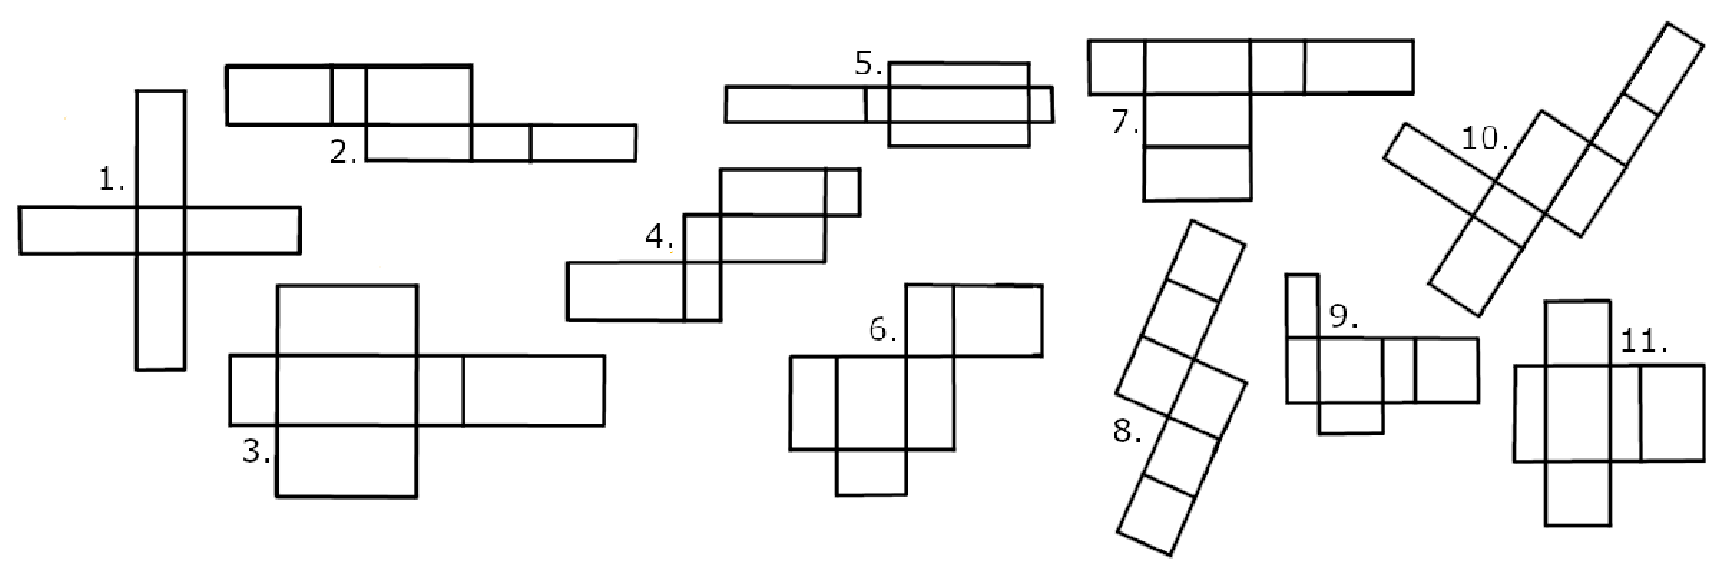
\includegraphics[width=16cm]{patrons_paves}
   \end{center}
\end{exercice}

\begin{corrige}
   \begin{itemize}
      \item Les figures {\blue 2, 5, 6, 8; 9} sont des patrons de pavés.
      \item Les figures 1 et 10 n'ont pas le bon nombre de faces (5 et 7).
      \item Les figures 3, 4 et 11 possèdent des arêtes qui ne se correspondent pas.
      \item La figure 7 a deux faces qui se superposent.
   \end{itemize}
\end{corrige}

\bigskip


\begin{exercice} %5
   Parmi tous ces développements, quels sont ceux qui permettent de construire un cylindre ? \smallskip
   \begin{center}
      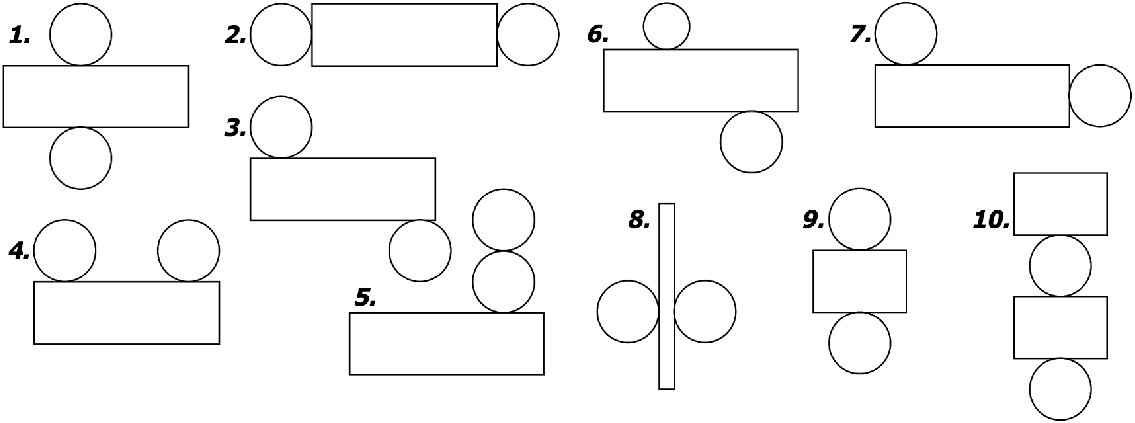
\includegraphics[width=16cm]{patrons_cylindres}
   \end{center}
\end{exercice}

\begin{corrige}
   \begin{itemize}
      \item Les figures {\blue 1, 3, 8 et 10 sont les développements de cylindres} (la figure 10 est un cas particulier avec une surface divisée en deux parties).
      \item Les figures 2 et 9 possèdent un rectangle trop court par rapport au périmètre du disque.
      \item Les figures 4, 5 et 7 ont un disque mal placé.
      \item La figure 6 possède un disque trop petit.
   \end{itemize}
\end{corrige}


%%%%%%%%%%%%%%%%%%%%%%%%%%%%%%%%%
%%%%%%%%%%%%%%%%%%%%%%%%%%%%%%%%%
\Recreation

\begin{enigme}[Des dessins magiques]


\hspace*{-10mm}
{\psset{unit=0.75}
\begin{pspicture*}(-1,-1)(24,27.5)
   \multido{\i=-15+1}{45}{\rput(\i;90){\multido{\n=0+1}{29}{\psdot[linewidth=0.05mm,linecolor=gray](\n;30)}}} % quadrillage
   \cubiso{1.732}{1}
   \cubiso{5.196}{1}
   \cubiso{8.66}{1}
   \cubiso{3.464}{4}
   \cubiso{6.928}{4}
   \cubiso{5.196}{7}
   \rput(0,18){ % trident
      \psline(0,0)(19;30)(23.383,5.5)(8;-30)
      \psline(0,-2)(16.454,7.5)(19.919,5.5)(3.464,-4)
      \psline(23.383,5.5)(23.383,3.5)(6.928,-6)
      \psline(16.454,7.5)(16.454,5.5)(18.187,4.5)
      \psline(16.454,5.5)(3.464,-2)
      \psellipse(0,-1)(0.4,0.98)
      \psellipse(3.464,-3)(0.4,0.98)
      \psellipse(6.928,-5)(0.4,0.98)
   }
   \psset{fillstyle=solid,fillcolor=teal}
   \rput(3.464,-2){\pspolygon(2;90)(2;30)(4;30)(3.464;60)}
   \rput(6.928,-2){\pspolygon(2;90)(2;30)(4;30)(3.464;60)}
   \psset{fillcolor=purple!80}
   \rput(8.66,7){\pspolygon(0,0)(2;90)(2;30)(2;-30)}
   \rput(10.393,4){\pspolygon(0,0)(2;90)(2;30)(2;-30)}
   \psset{fillcolor=lightgray}
   \rput(0,4){\pspolygon(2;-30)(3.464;0)(4;30)(2;30)}
   \rput(1.732,7){\pspolygon(2;-30)(3.464;0)(4;30)(2;30)}
   \rput(17;30){ %triangle impossible
      \pspolygon[fillcolor=cyan](0,0)(8;-30)(7.794,-3.5)(1.732,0)(6.062,2.5)(6.062,3.5)(7;30)
      \pspolygon[fillcolor=violet](0,0)(7;30)(6.062,-1.5)(6.928,-2)(6.928,5)(1;90)
      \pspolygon[fillcolor=orange](1.732,0)(7.794,-3.5)(7.794,4.5)(6.928,5)(6.928,-2)(2.598,0.5)
   }
   \psframe[fillstyle=solid,fillcolor=white,linecolor=white](0,25)(6,27.5)
   \rput(3,26.6){Reproduire ces dessins}
   \rput(3,25.8){sur du papier pointé}
\end{pspicture*}}

\pagebreak

\hspace*{-10mm}
{\psset{unit=0.75}
\begin{pspicture*}(-1,-1)(24,28)
   \multido{\i=-15+1}{45}{\rput(\i;90){\multido{\n=0+1}{29}{\psdot[linewidth=0.05mm,linecolor=gray](\n;30)}}}
\end{pspicture*}}
\end{enigme}

